\subsection{ACM}
\label{subsec:acm}
\begin{tcoloritemize}
    \blueitem[ACM]
    \textbf{A}ir \textbf{C}ombat \textbf{M}ode

    \begin{itemize}
        \item \textbf{Used to automatically lock targets while maneuvering}
        \item \textbf{Sub-Modes}
        \begin{itemize}
            \item \textbf{HUD Scan} --- 30x20 deg 
            \item \textbf{BORE} --- Boresight (3x3 deg)
            \item \textbf{Vertical Scan} --- 10x60 deg
            \item \textbf{Slewable} --- WIP
        \end{itemize}
    \end{itemize}
\end{tcoloritemize}

\begin{figure}[htbp]
    \centering
    \begin{tikzpicture}[auto, node distance=10mm, x=1mm, y=1mm, very thick,
        >={Latex[round]}
        ]
        
        % \node[<options>](<coordinate name>)at(<coordinate>){<text>};
        \node[
            hyperref node=subsec:acm,
            rectangle,
            rounded corners,
            minimum width=15mm,
            minimum height=15mm,
            draw,
        ](acm)at(0,0){\blue{ACM}};
        \node[
            rectangle,
            rounded corners,
            minimum width=20mm,
            minimum height=7.5mm,
            draw,
        ](bore)at(0,20){\textbf{BORE}};
        \node[
            rectangle,
            rounded corners,
            minimum width=20mm,
            minimum height=7.5mm,
            draw,
        ](hud)at(32.5,0){\textbf{HUD}};
        \node[
            rectangle,
            rounded corners,
            minimum width=20mm,
            minimum height=7.5mm,
            draw,
        ](vert)at(0,-20){\textbf{Vertical}};
        \node[
            hyperref node=subsec:stt,
            rectangle, 
            rounded corners,
            minimum width=90mm,
            minimum height=7.5mm,
            draw, 
        ](stt)at(0,35){\blue{STT}};
                
        % Lines
        \draw [->]
            (acm) -- node[pos=0.5, left]{\scriptsize\textbf{TMS FWD}} (bore);
        \draw [->]
            (acm) -- node[pos=0.5, above]{\scriptsize\textbf{TMS}}node[pos=0.5, below]{\scriptsize\textbf{RIGHT}} (hud);
        \draw [->]
            (acm) -- node[pos=0.5, left]{\scriptsize\textbf{TMS AFT}} (vert);
        \draw [->]
            let
                \p1=(bore.north),
                \p2=(stt.south),
            in
                (\p1) -- node[pos=0.5, left]{\scriptsize\textbf{Automatic}} (\x1,\y2);
        \draw [->]
            let
                \p1=(hud.north),
                \p2=(stt.south),
            in
                (\p1) -- node[pos=0.5, left]{\scriptsize\textbf{Automatic}} (\x1,\y2);
        \draw [->, rounded corners]
            let
                \p1=(vert.west),
                \p2=(stt.south),
            in
                (\p1) -- (\x1-22.5mm,\y1) -- node[pos=0.5, left]{\scriptsize\textbf{Automatic}} (\x1-22.5mm,\y2);
                
    \end{tikzpicture}
    \caption{ACM Radar Modes Overview}
    \label{fig:acmoverview}
\end{figure}

\begin{figure}[htbp]
    \centering
    \begin{tikzpicture}[auto, node distance=10mm, x=1mm, y=1mm, very thick, line cap=round,
        >={Latex[round]}
        ]
        
        \node[] (fig) at (0,0) {
            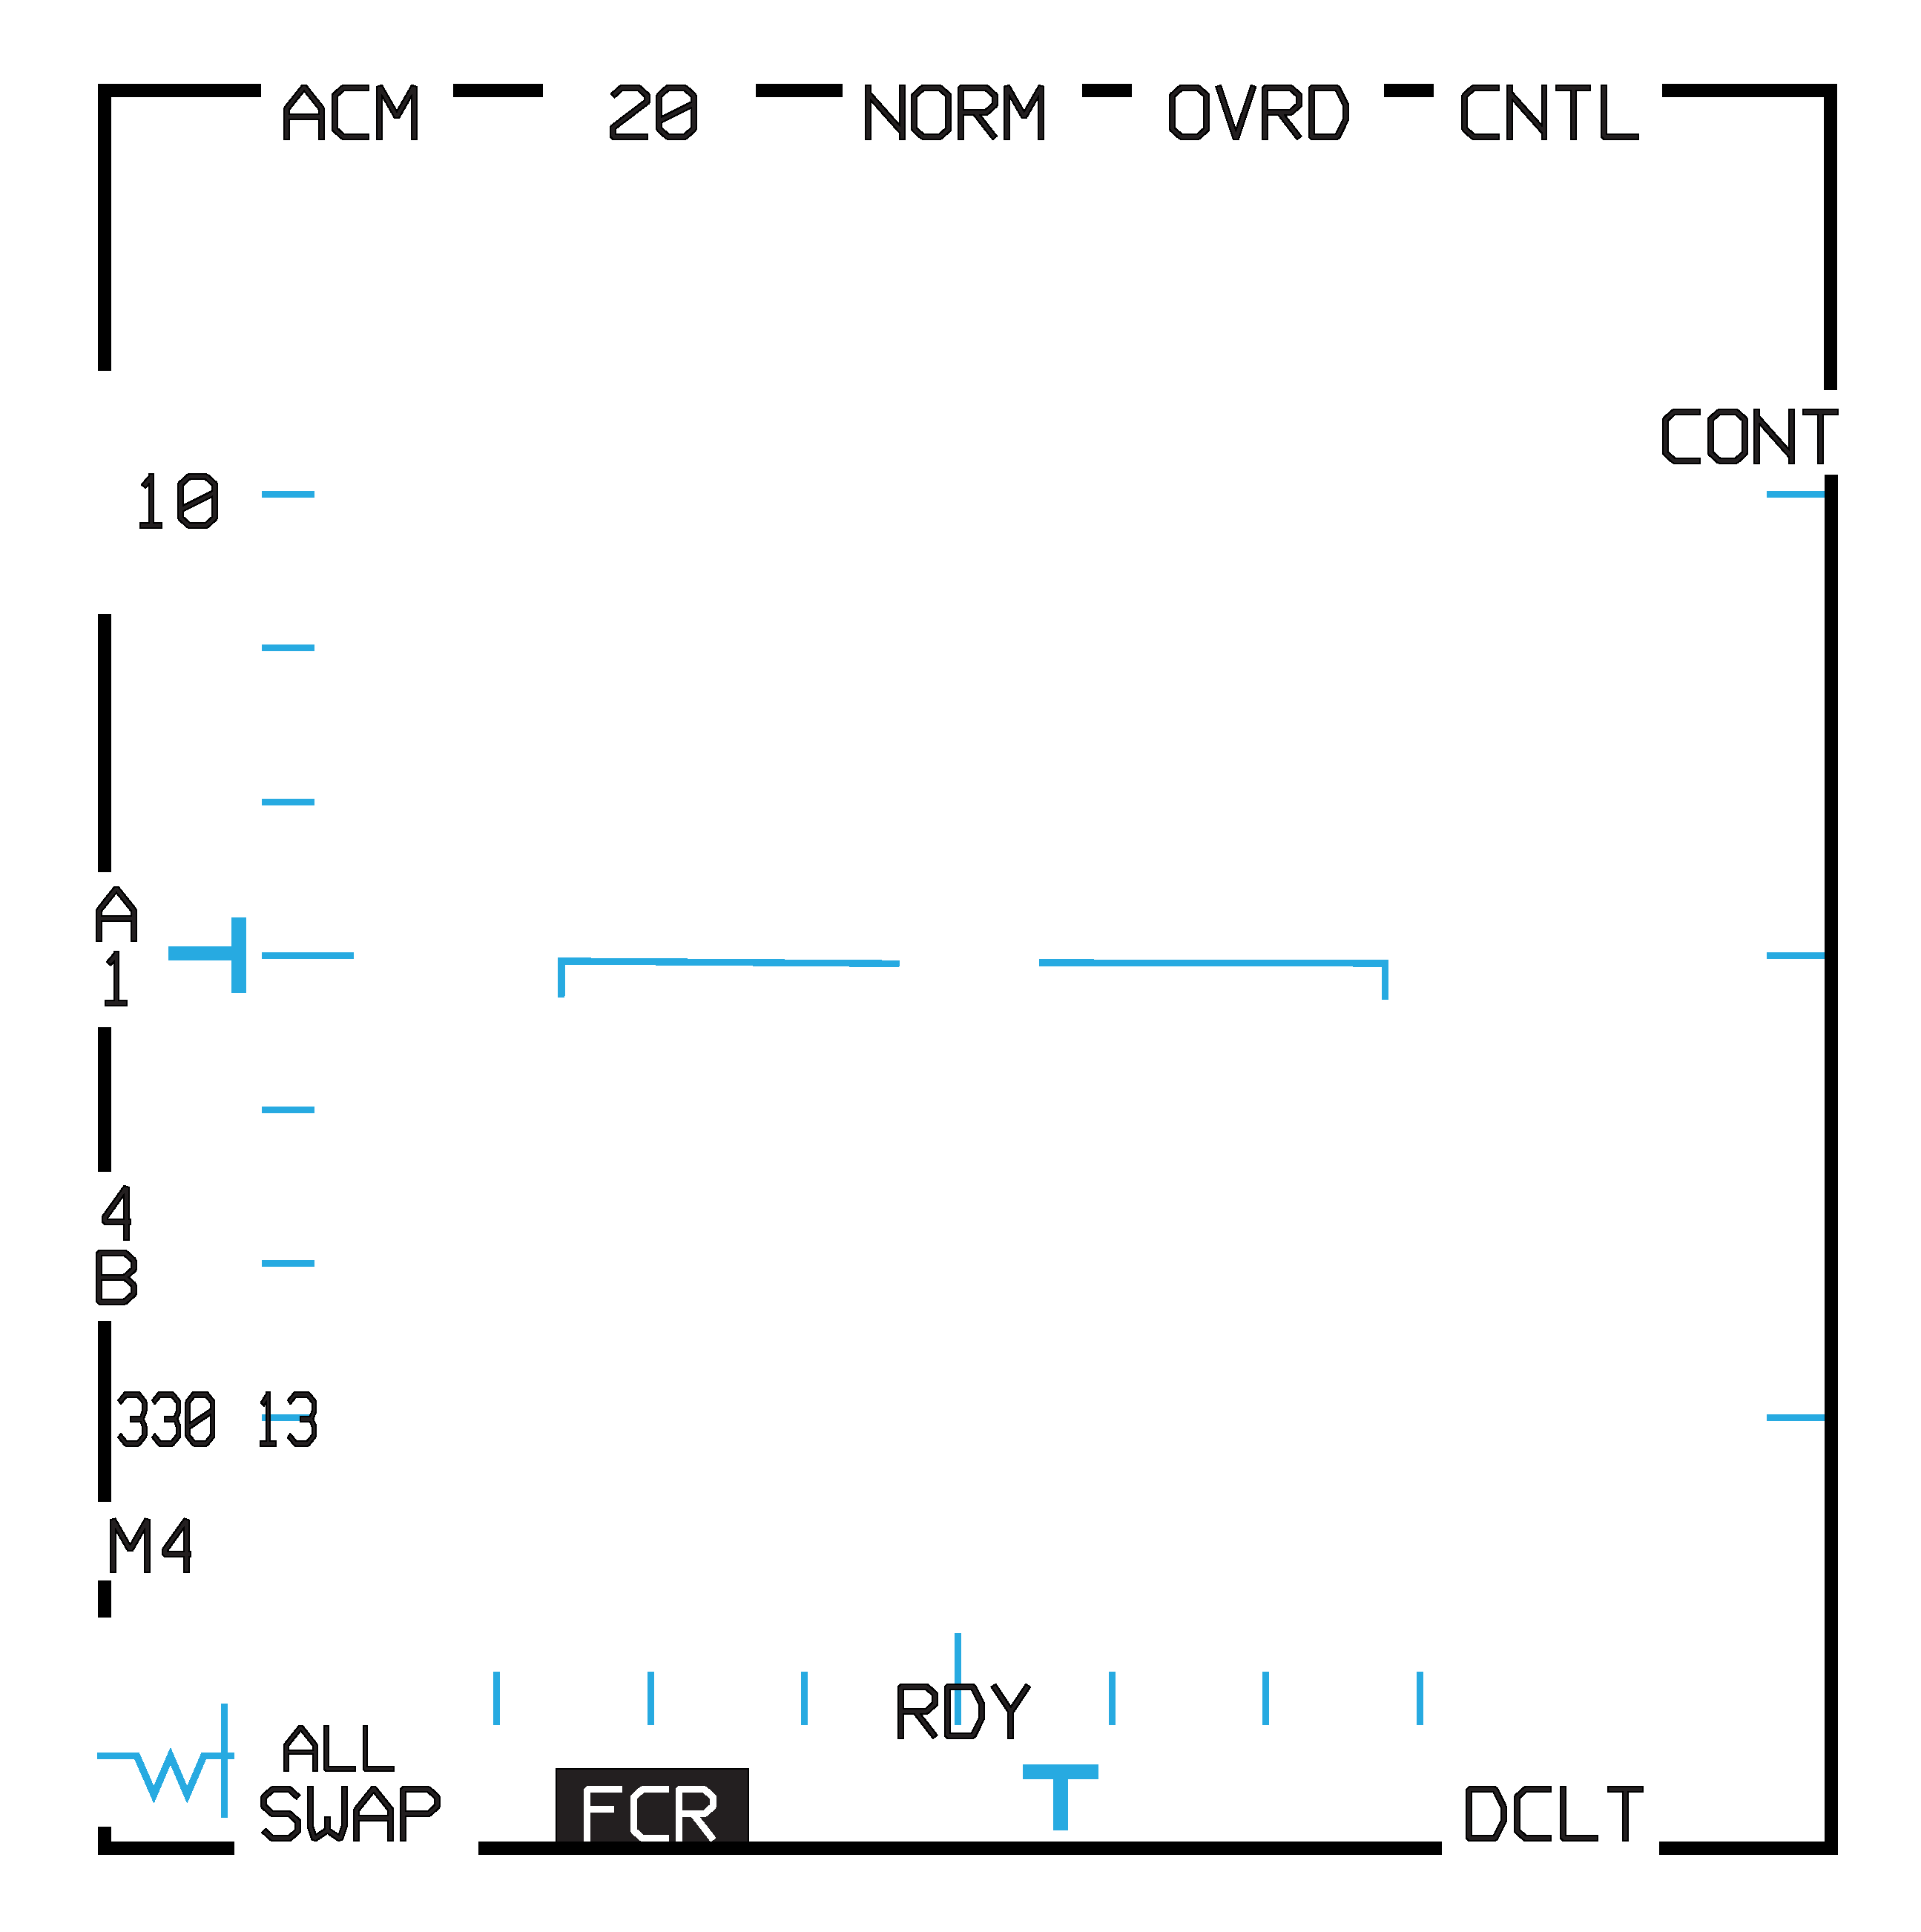
\includegraphics[
                height=75mm,
            ]{mfd/fcr_aa/acm_homepage.pdf}
        };

        % Annotations
        \node[lannot] (mode) at ($(fig.west)+(0mm,38mm)$) {FCR mode};
        \draw[annotptr] (mode.east) -- ++(12mm, 0mm) -- (-24mm,35mm);

        \node[lannot] (submode) at ($(fig.west)+(0mm,28mm)$) {ACM \\ submode};
        \draw[annotptr] (submode.east) -- ++(23mm, 0mm) -- (-13mm, 31mm);

        \node[lannot] (rsel) at ($(fig.west)+(0mm,18mm)$) {Range scale};
        \draw[annotptr] (rsel.east) -- ++(4.5mm, 0mm);

        \node[lannot] (asel) at ($(fig.west)+(0mm,0.5mm)$) {Azimuth};
        \draw[annotptr] (asel.east) -- ++(4.5mm, 0mm);

        \node[lannot] (bsel) at ($(fig.west)+(0mm,-10.5mm)$) {Elevation \\ bar};
        \draw[annotptr] (bsel.east) -- ++(4.5mm, 0mm);

        \node[annot, anchor=south, align=center] (fov) at ($(fig.north)+(0mm,0mm)$) {FOV select};
        \draw[annotptr] (fov.south) -- ++(0mm, -3.5mm);

        \node[rannot] (cntl) at ($(fig.east)+(0mm,38mm)$) {Control};
        \draw[annotptr] (cntl.west) -- ++(-13mm, 0mm) -- (23mm, 35mm);

        \node[rannot] (ovrd) at ($(fig.east)+(0mm,28mm)$) {Override};
        \draw[annotptr] (ovrd.west) -- ++(-24mm, 0mm) -- (12mm, 31mm);

        \node[rannot] (dl) at ($(fig.east)+(0mm,20.5mm)$) {Datalink mode};
        \draw[annotptr] (dl.west) -- ++(-4mm,0mm);

        \node[rannot] (sj) at ($(fig.east)+(0mm,-8mm)$) {Horizon \\indicator};
        \draw[annotptr] (sj.west) -- ++(-20mm, 0mm) -- (12mm,-1mm);

        \node[rannot] (dclt) at ($(fig.east)+(0mm,-38mm)$) {Declutter};
        \draw[annotptr] (dclt.west) -- ++(-13mm, 0mm) -- (23mm, -35mm);
    \end{tikzpicture}
    \caption{ACM FCR page symbology}
\end{figure}

\begin{figure}[htbp]
    \centering
    \begin{subfigure}[t]{0.3\linewidth}
        \centering
        \begin{tikzpicture}[figstyle]
            
            \draw[color2, fill=color2!20, dashed, rounded corners]
            (-15, 10) -- (15,10) -- (15,-10) -- (-15,-10) -- cycle;

            \node[] (fig) at (0,0) {
                
\includegraphics[
                    scale=0.25,
                ]{hud/acm/subfig_hud.pdf}
            };

        \end{tikzpicture}
        \caption{HUD}
    \end{subfigure}
    \begin{subfigure}[t]{0.3\linewidth}
        \centering
        \begin{tikzpicture}[figstyle]

            \draw[color2, fill=color2!20, dashed] 
            (0,-3) circle [x radius=4, y radius=6];
            
            \node[] (bore) at (0,0) {
                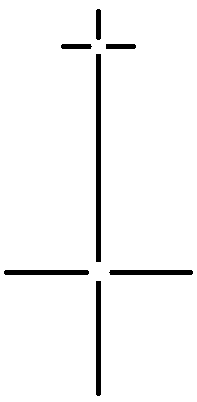
\includegraphics[
                    scale=0.25,
                ]{hud/acm/subfig_bore.pdf}
            };
    
        \end{tikzpicture}
        \caption{BORE}
    \end{subfigure}
    \begin{subfigure}[t]{0.3\linewidth}
        \centering
        \begin{tikzpicture}[figstyle]

            \draw[color2, fill=color2!20, dashed, rounded corners]
            (-2.5, 30) -- (2.5,30) -- (2.5,-8) -- (-2.5,-8) -- cycle;
            
            \node[] (vert) at (0,0) {
                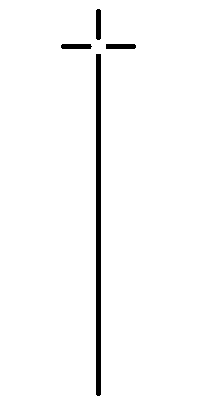
\includegraphics[
                    scale=0.25,
                ]{hud/acm/subfig_vert.pdf}
            };
    
        \end{tikzpicture}
        \caption{Vertical}
    \end{subfigure}
    \caption{
        ACM Scan Patterns shown with the relevant HUD symbology. 
        The dashed lines indicate the scan volume for illustrative purposes and are not to scale.
    }
\end{figure}

\begin{figure}[htbp]
    \centering
    \begin{tikzpicture}[auto, node distance=10mm, x=1mm, y=1mm, very thick, line cap=round,
        >={Latex[round]}
        ]

        \node[draw, rounded corners] (fig) at (0,0) {
            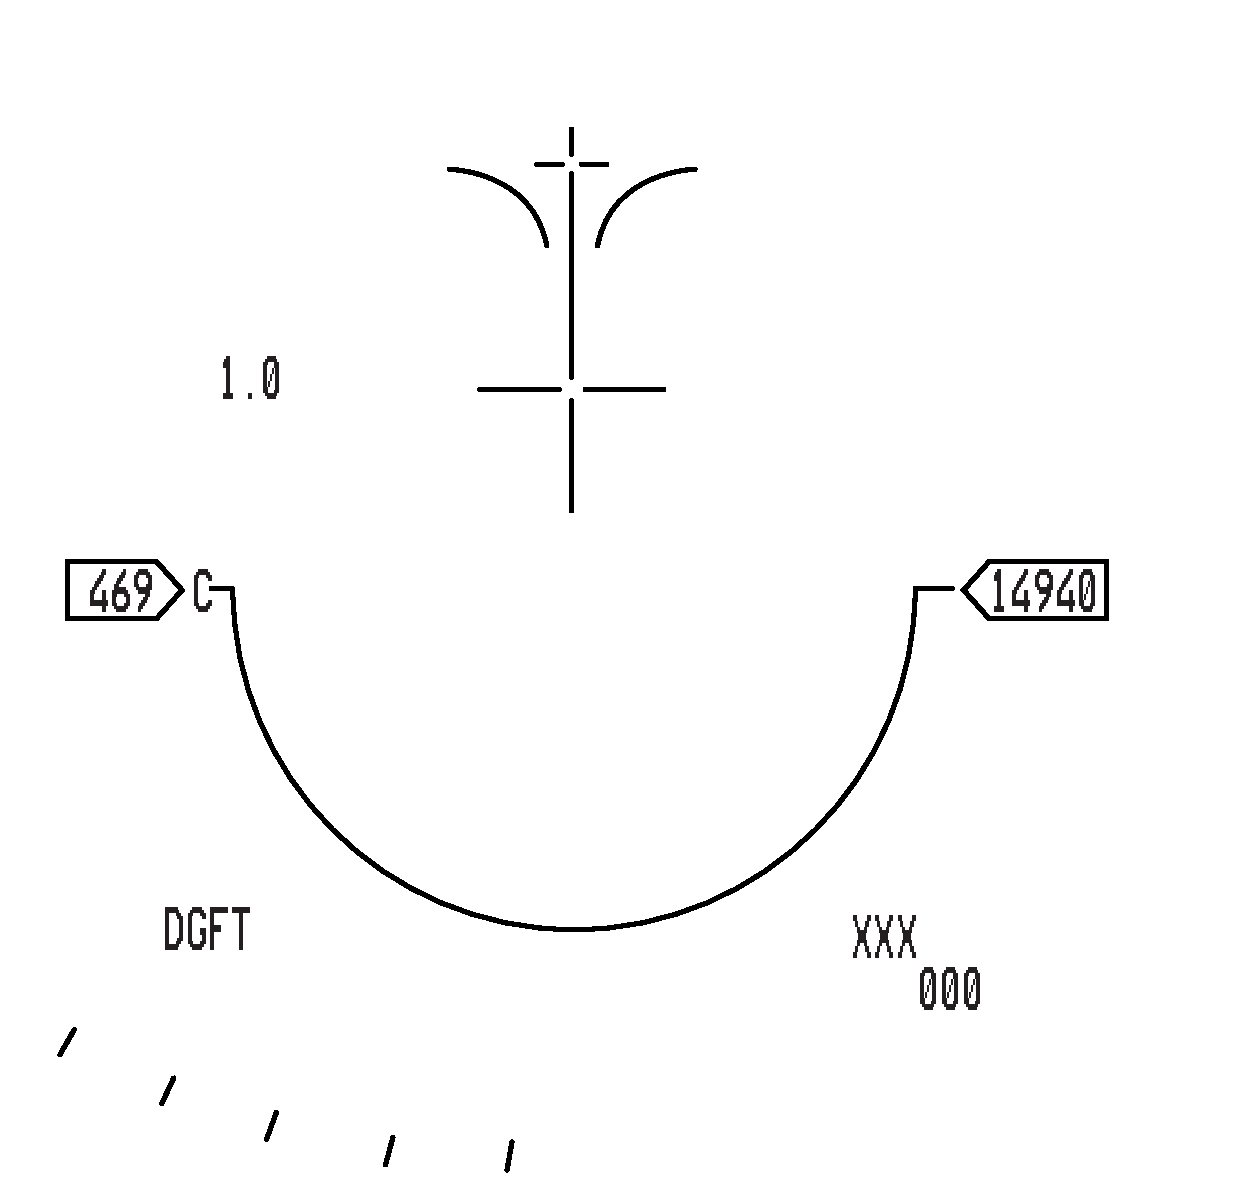
\includegraphics[
                height=75mm,
            ]{hud/acm/bore.pdf}
        };

        % Annotations
        \node[lannot] (bs) at ($(fig.west)+(-2.5mm,34mm)$) {Boresight cross};
        \draw[annotptr] (bs.east) -- ++(34mm,0mm) -- ++(4mm,-4mm);

        \node[lannot] (eegs) at ($(fig.west)+(-2.5mm,24mm)$) {EEGS funnel};
        \draw[annotptr] (eegs.east) -- ++(32mm,0mm);

        \node[lannot] (acc) at ($(fig.west)+(-2.5mm,13.5mm)$) {Acceleration};
        \draw[annotptr] (acc.east) -- ++(16mm,0mm);

        \node[lannot] (cas) at ($(fig.west)+(-2.5mm,0mm)$) {Airspeed \\ {\footnotesize calibrated}};
        \draw[annotptr] (cas.east) -- ++(7mm,0mm);

        \node[lannot] (dgft) at ($(fig.west)+(-2.5mm,-15mm)$) {Mode};
        \draw[annotptr] (dgft.east) -- ++(9mm,0mm) -- ++(4mm, -4mm);

        \node[lannot] (mgrs) at ($(fig.west)+(-2.5mm,-32mm)$) {MGRS lines};
        \draw[annotptr] (mgrs.east) -- ++(10mm,0mm);

        \node[rannot] (bore) at ($(fig.east)+(2.5mm,13mm)$) {Scan zone indicator};
        \draw[annotptr] (bore.west) -- ++(-38mm, 0mm);

        \node[rannot] (alt) at ($(fig.east)+(2.5mm,0mm)$) {Altimeter};
        \draw[annotptr] (alt.west) -- ++(-12mm, 0mm);

        \node[rannot] (arc) at ($(fig.east)+(2.5mm,-12mm)$) {Attitude arc};
        \draw[annotptr] (arc.west) -- ++(-28mm, 0mm);

        \node[rannot] (slant) at ($(fig.east)+(2.5mm,-25.25mm)$) {Target slant range};
        \draw[annotptr] (slant.west) -- ++(-20mm, 0mm);
    \end{tikzpicture}
    \caption{ACM HUD Symbology. Shown in BORE submode.}
\end{figure}

\begin{figure}[htbp]
    \centering
    \begin{tikzpicture}[auto, node distance=10mm, x=1mm, y=1mm, very thick, line cap=round,
        >={Latex[round]}
        ]

        \node[draw, rounded corners] (fig) at (0,0) {
            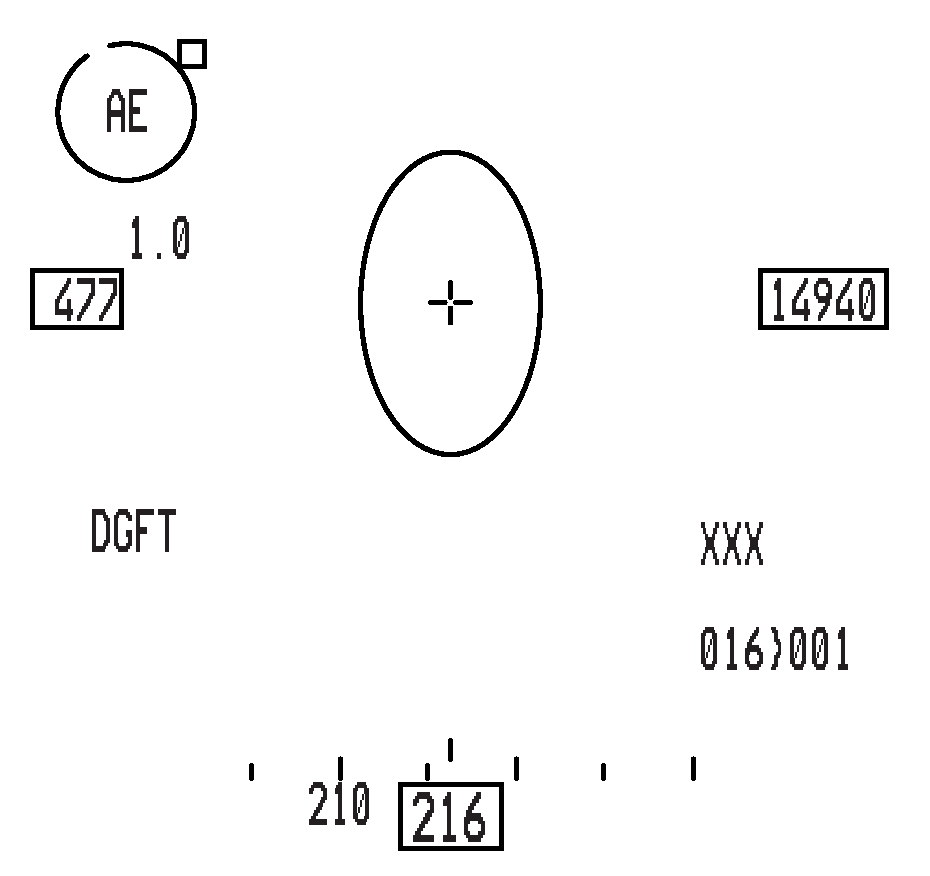
\includegraphics[
                height=60mm,
            ]{hmd/dgft.pdf}
        };

        % Annotations
        \node[lannot] (rwr) at ($(fig.west)+(-2.5mm,22.5mm)$) {RWR};
        \draw[annotptr] (rwr.east) -- ++(7mm,0mm);

        \node[lannot] (acc) at ($(fig.west)+(-2.5mm,16.5mm)$) {Acceleration};
        \draw[annotptr] (acc.east) -- ++(8mm,0mm) -- ++(4mm, -2mm);

        \node[lannot] (cas) at ($(fig.west)+(-2.5mm,9.5mm)$) {Airspeed};
        \draw[annotptr] (cas.east) -- ++(5.5mm,0mm);

        \node[lannot] (cross) at ($(fig.west)+(-2.5mm,2mm)$) {Aiming cross};
        \draw[annotptr] (cross.east) -- ++(28mm,0mm) -- ++(5mm,5mm);

        \node[lannot] (dgft) at ($(fig.west)+(-2.5mm,-6.5mm)$) {Mode};
        \draw[annotptr] (dgft.east) -- ++(7mm,0mm);

        \node[lannot] (hdg) at ($(fig.west)+(-2.5mm,-26mm)$) {Heading \\ {\footnotesize HMD LOS}};
        \draw[annotptr] (hdg.east) -- ++(22mm,0mm);

        \node[rannot] (acq) at ($(fig.east)+(2.5mm,22.5mm)$) {Acquisition circle};
        \draw[annotptr] (acq.west) -- ++(-28mm,0mm) -- ++(-4mm,-4mm);

        \node[rannot] (alt) at ($(fig.east)+(2.5mm,9.5mm)$) {Altimeter};
        \draw[annotptr] (alt.west) -- ++(-6mm, 0mm);

        \node[rannot] (range) at ($(fig.east)+(2.5mm,-1mm)$) {Target slant range};
        \draw[annotptr] (range.west) -- ++(-10mm, 0mm) -- ++(-4mm, -4mm);

        \node[rannot] (stpt) at ($(fig.east)+(2.5mm,-14.5mm)$) {Distance to STPT};
        \draw[annotptr] (stpt.west) -- ++(-8mm, 0mm);
    \end{tikzpicture}
    \caption{
        ACM HMD Symbology. 
        Shown in BORE submode. 
        Note that RWR indication is of highest threat 
        with diamond indicating direction of threat 
        and gap indicating current HMD LOS.
    }
\end{figure}

\begin{tcoloritemize}
    \blueitem[HUD Submode]
    \begin{itemize}
        \item \textbf{30x20 deg scan} --- slightly larger than HUD
        \item \textbf{Lock Range} --- 10 nm
        \item \textbf{Selected with TMS Right} --- default mode upon ACM selection
        \item \textbf{Default ACM mode} --- but in \textbf{NO RAD} (non-radiating) state
        \item \textbf{Displays}
        \begin{itemize}
            \item \textbf{FCR Format} --- displays \textbf{ACM 20}
            \item \textbf{HUD} --- no special symbology
        \end{itemize}
    \end{itemize}
    \blueitem[BORE Submode]
    \begin{itemize}
        \item \textbf{Small, 1-beamwidth scan}
        \begin{itemize}
            \item centered 3 deg below gun cross
            \item useful for precisely locking up target
        \end{itemize}
        \item \textbf{Lock Range} --- 20 nm
        \item \textbf{Selected with TMS Forward}
        \item \textbf{Scan slaves to HMD} (if equipped and powered)
        \item \textbf{Displays}
        \begin{itemize}
            \item \textbf{FCR Format} --- displays \textbf{ACM BORE}
            \item \textbf{HUD} --- Boresight Cross at center of radar scan zone
            \item \textbf{HMD} --- Oval centered on HMD aiming cross
        \end{itemize}
    \end{itemize}
    \blueitem[Vertical \break Submode]
    \begin{itemize}
        \item \textbf{10x60 deg scan}
        \begin{itemize}
            \item centered 23 deg above gun cross
            \item useful during turning engagement to lock target ``across the circle''
        \end{itemize}
        \item \textbf{Lock Range} --- 10 nm
        \item \textbf{Selected with TMS Aft}
        \item \textbf{Displays}
        \begin{itemize}
            \item \textbf{FCR Format} --- displays \textbf{ACM 60}
            \item \textbf{HUD} --- Vertical line
        \end{itemize}
    \end{itemize}
    \blueitem[Slewable \break Submode --- WIP]
    \begin{itemize}
        \item \textbf{Scan} --- WIP
        \item \textbf{Lock Range} --- WIP
        \item \textbf{Slew} --- \textbf{CURSOR/ENABLE Control}
        \item \textbf{Displays}
        \begin{itemize}
            \item \textbf{FCR Format} --- displays \textbf{ACM SLEW}
            \item \textbf{HUD} --- WIP
        \end{itemize}
    \end{itemize}
    \blueitem[NO RAD]
    Upon selection of \textbf{ACM} or dropping target lock the radar is placed in non-radiating state
\end{tcoloritemize}

\marginfigeometry

\subsubsection{HUD / BORE / VERTICAL ACQUISITION}
\begin{checklistenumerate}
    \blueitem[FCR Setup]
    \marginpar{
        \captionsetup{type=figure}
        \begin{subfigure}[t]{\linewidth}
            \centering
            \begin{tikzpicture}[auto, node distance=10mm, x=1mm, y=1mm, very thick, line cap=round,
                >={Latex[round]}
                ]
    
                \draw[color2, fill=color2!20, dashed, rounded corners]
                (-15, 10) -- (15,10) -- (15,-10) -- (-15,-10) -- cycle;
                
                \node[] (hud) at (0,0) {
                    
\includegraphics[
                        scale=0.25,
                    ]{hud/acm/subfig_hud.pdf}
                };
        
            \end{tikzpicture}
            \caption{HUD}
        \end{subfigure}
        \begin{subfigure}[t]{0.45\linewidth}
            \centering
            \begin{tikzpicture}[auto, node distance=10mm, x=1mm, y=1mm, very thick, line cap=round,
                >={Latex[round]}
                ]
    
                \draw[color2, fill=color2!20, dashed] 
                (0,-3) circle [x radius=4, y radius=6];
                
                \node[] (bore) at (0,0) {
                    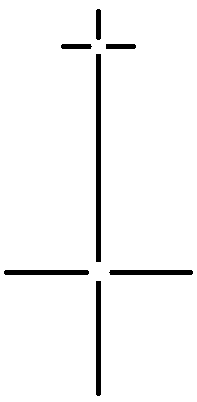
\includegraphics[
                        scale=0.25,
                    ]{hud/acm/subfig_bore.pdf}
                };
        
            \end{tikzpicture}
            \caption{BORE}
        \end{subfigure}
        \begin{subfigure}[t]{0.45\linewidth}
            \centering
            \begin{tikzpicture}[auto, node distance=10mm, x=1mm, y=1mm, very thick, line cap=round,
                >={Latex[round]}
                ]
    
                \draw[color2, fill=color2!20, dashed, rounded corners]
                (-2.5, 30) -- (2.5,30) -- (2.5,-8) -- (-2.5,-8) -- cycle;
                
                \node[] (vert) at (0,0) {
                    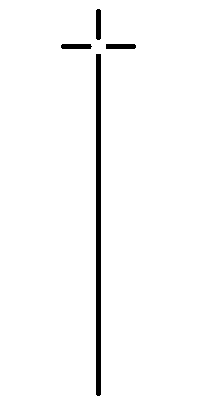
\includegraphics[
                        scale=0.25,
                    ]{hud/acm/subfig_vert.pdf}
                };
        
            \end{tikzpicture}
            \caption{Vertical}
        \end{subfigure}
        \caption{HUD / BORE / VERTICAL Symbology}
    }
    \begin{enumerate}
        \item \textbf{FCR Switch} \dotfill \textbf{FCR}
        \item \textbf{Desired MFD} \dotfill \textbf{FCR Page}
    \end{enumerate}
    \blueitem[Enter ACM]
    \begin{enumerate}
        \item \textbf{Dogfight/Missile Override} \dotfill \textbf{DGFT}
        \item \textbf{Radar Mode (OSB 2)} \dotfill verify \textbf{ACM}
    \end{enumerate}
    \blueitem[Select ACM Submode]
    \begin{itemize}
        \item \textbf{HUD} (default ACM mode) \dotfill \textbf{TMS Right}
        \item \textbf{Bore} \dotfill \textbf{TMS Forward}
        \item \textbf{Vertical} \dotfill \textbf{TMS Aft}
    \end{itemize}
    \blueitem[Target Acquisition]
    \begin{enumerate}
        \item Maneuver aircraft to place target within selected ACM scan volume 
        \item Wait for automatic transition to STT 
    \end{enumerate}
    \blueitem[Target Rejection]
    To unlock target
    \begin{enumerate}
        \item \textbf{TMS} \dotfill \textbf{Aft}
    \end{enumerate}
    Radar returns to \textbf{HUD} submode in \textbf{NO RAD} 
    
\end{checklistenumerate}

\subsubsection{HMD ACQUISITION}
\begin{checklistenumerate}
    \blueitem[FCR/MFD Setup]
    \marginpar{
        \captionsetup{type=figure}
        \centering
        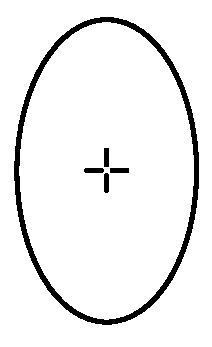
\includegraphics[
            height=25mm,
        ]{hmd/dgft_subfig_bore.pdf}
        \caption{HMD acquisition circle}
    }
    \begin{enumerate}
        \item \textbf{FCR Switch} \dotfill \textbf{FCR}
        \item \textbf{Desired MFD} \dotfill \textbf{FCR Page}
        \item \textbf{HMD Brightness} \dotfill \textbf{On}
    \end{enumerate}
    \blueitem[Enter ACM]
    \begin{enumerate}
        \item \textbf{Dogfight/Missile Override} \dotfill \textbf{DGFT}
        \item \textbf{Radar Mode (OSB 2)} \dotfill verify \textbf{ACM}
    \end{enumerate}
    \blueitem[Select ACM Bore Submode]
    \begin{itemize}
        \item \textbf{Bore} \dotfill \textbf{TMS Forward}
    \end{itemize}
    \blueitem[Target Acquisition]
    \begin{enumerate}
        \item Maneuver aircraft to place target within 60 deg of nose 
        \item Place target within HMD acquisition circle
        \item Wait for automatic transition to STT 
    \end{enumerate}
    \blueitem[Target Rejection]
    To unlock target
    \begin{enumerate}
        \item \textbf{TMS} \dotfill \textbf{Aft}
    \end{enumerate}
    Radar returns to \textbf{HUD} submode in \textbf{NO RAD}
\end{checklistenumerate}

\subsubsection{SLEWABLE ACQUISITION --- WIP}

\marginfigrestore